\documentclass[10pt, a4paper]{scrartcl}

\usepackage{vorschule}
\usepackage[
	typ=ab,
	fach=Informatik,
	lerngruppe={IF-GK},
	nummer=3,
	module={Symbole,Lizenzen},
	seitenzahlen=keine,
	farbig,
	lizenz=cc-by-nc-sa-4,
]{schule}

\usepackage[ 
	kuerzel=Ngb,
	reihe={Relationale Datenbanken},
	version={2020-08-25},
]{ngbschule}

\author{J. Neugebauer}
\title{ERM transformieren}
\date{\Heute}

\setzeAufgabentemplate{ngbnormal}


\begin{document}
\ReiheTitel

Wenn der erste Entwurf einer Datenbank in Form eines ER-Diagramms erstellt wurde, muss dieses im nächsten Schritt
in ein \emph{Relationenschema} transformiert werden. Ein \emph{Relationenschema} beschreibt die \emph{Relationen} 
(d.h. Tabellen), aus denen die relationale Datenbank am Ende bestehen soll.

Eine Relation wird in einem festen Format beschrieben:
\begin{center}\rmfamily
Name(\underline{Schlüsselattribut}, Attribut 1, Attribut2, ...)
\end{center}


Die Transformation findet in vier Schritten (nach vier \emph{Regelen}) statt:
\begin{enumerate}
	\item\begin{multicols}{2}
		Jede \emph{Entität} mit ihren \emph{Attributen} wird eine Relation.
		
		\begin{center}
		\begin{tikzpicture}
			\node (Buch) at (0,0) [entity] {Buch};
			\node (ISBN) at (-2,0) [attribute] {\underline{ISBN}};
			\node (Titel) at (2,0) [attribute] {Titel};
			\draw (Buch) -- (ISBN);
			\draw (Buch) -- (Titel);
		\end{tikzpicture}
		\end{center}
		
		\code{Buch(\underline{ISBN}, Titel)}
	\end{multicols} 
		
	\item\begin{multicols}{2}
		 Jede \code{m:n}-Beziehung wird in eine eigenständige Relation überführt. Als Attribute bekommt die neue Relation die \emph{Primärschlüssel} der beiden verknüpften \emph{Entitäten}. Die Menge dieser Schlüsselattribute bildet den Primärschlüssel dieser Relation. Zusätzlich werden die Attribute der Relation aufgenommen.
		
		\begin{center}
		\begin{tikzpicture}[node distance=1cm]
			\node (Buch)  at (-2,0) [entity] {Buch};
			\node (ISBN)  at (-2,1) [attribute] {\underline{ISBN}};
			\node (Titel)  at (-2,-1) [attribute] {Titel};
			\draw (Buch) -- (ISBN);
			\draw (Buch) -- (Titel);
			
			\node (kauft) at (0,0) [relation] {kauft};
			\node (Anzahl) at (0,1) [attribute] {Anzahl};
			\draw (kauft) -- (Anzahl);
			
			\node (Kunde) at (2,0) [entity] {Kunde};
			\node (KID) at (2,1) [attribute] {\underline{KID}};
			\node (Name) at (2,-1) [attribute] {Name};
			\draw (Kunde) -- (KID);
			\draw (Kunde) -- (Name);
			
			\draw (Buch) --node[above]{m} (kauft) --node[above]{n} (Kunde);
		\end{tikzpicture}
		\end{center}
		
		\code{kauft(\foreignkey\underline{KID}, \foreignkey\underline{ISBN}, Anzahl)}
	\end{multicols} 
	
	\item\begin{multicols}{2}
		 Jede \code{1:n}-Beziehung wird ohne eigene Tabelle abgebildet. Statt dessen wird der Relation der Entität mit der Kardinalität \code{n} der \emph{Primärschlüssel} der anderen Entität als Attribut hinzugefügt.
		
		\begin{center}
		\begin{tikzpicture}[node distance=1cm]
			\node (Buch)  at (-2,0) [entity] {Buch};
			\node (ISBN)  at (-2,1) [attribute] {\underline{ISBN}};
			\node (Titel)  at (-2,-1) [attribute] {Titel};
			\draw (Buch) -- (ISBN);
			\draw (Buch) -- (Titel);
			
			\node (verlegt) at (0,0) [relation] {verlegt};
			
			\node (Verlag) at (2,0) [entity] {Verlag};
			\node (VID) at (2,1) [attribute] {\underline{VID}};
			\node (Name) at (2,-1) [attribute] {Name};
			\draw (Verlag) -- (VID);
			\draw (Verlag) -- (Name);
			
			\draw (Buch) --node[above]{n} (verlegt) --node[above]{1} (Verlag);
		\end{tikzpicture}
		\end{center}
		
		\code{Buch(\underline{ISBN}, Titel, \foreignkey VID)}
	\end{multicols} 
	
	\item\begin{multicols}{2}
		Jede \code{1:1}-Beziehung wird ohne eigene Tabelle abgebildet. Dazu wird der Primärschlüssel \emph{einer} Entität der Relation der anderen als Attribut hinzugefügt. \columnbreak
	
		\begin{center}
		\begin{tikzpicture}[node distance=1cm]
			\node (Mitarbeiter)  at (-2.5,0) [entity] {Mitarbeiter};
			\node (MID)  at (-2.5,1) [attribute] {\underline{MID}};
			\node (Nachname)  at (-2.5,-1) [attribute] {Nachname};
			\draw (Mitarbeiter) -- (MID);
			\draw (Mitarbeiter) -- (Nachname);
			
			\node (ceo) at (0,0) [relation] {ist CEO};
			
			\node (Verlag) at (2,0) [entity] {Verlag};
			\node (VID) at (2,1) [attribute] {\underline{VID}};
			\node (Name) at (2,-1) [attribute] {Name};
			\draw (Verlag) -- (VID);
			\draw (Verlag) -- (Name);
			
			\draw (Mitarbeiter) --node[above]{1} (ceo) --node[above]{1} (Verlag);
		\end{tikzpicture}
		\end{center}
		
		\code{Mitarbeiter(\underline{MID}, Nachname, \foreignkey VID)}
		
		\emph{oder}
		
		\code{Verlag(\underline{VID}, Name, \foreignkey MID)}
		\end{multicols} 
\end{enumerate}

\begin{aufgabe}
	Transformiere die drei ER-Diagramme mit den vier Regeln jeweils in ein \emph{Relationenschema}.
	\begin{center}
	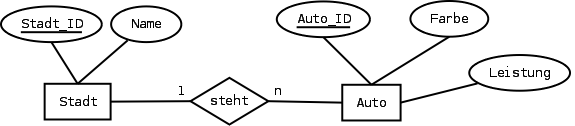
\includegraphics[width=12cm]{Q2-AB.3-Abb_ERD Autos}
	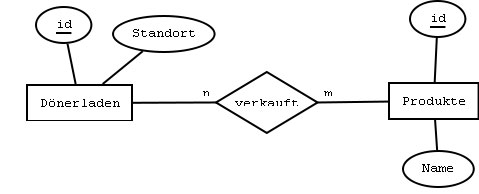
\includegraphics[width=12cm]{Q2-AB.3-Abb_ERD Doenerladen}
	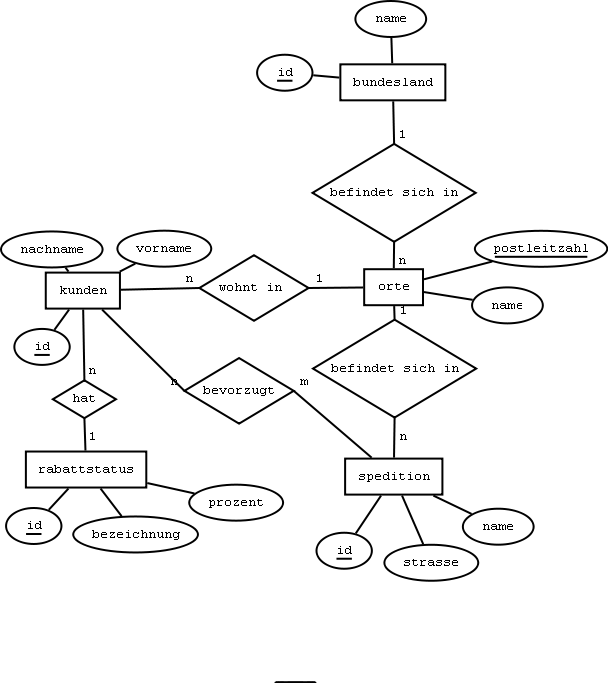
\includegraphics[width=12cm]{Q2-AB.3-Abb_ERD Spedition}
	\end{center}
\end{aufgabe}

\end{document}
